\section{Python's Standard Library}

\begin{frame}{Python's Standard Library}
\alert{``Batteries included''}: comprehensive standard library for various tasks\\[4mm]

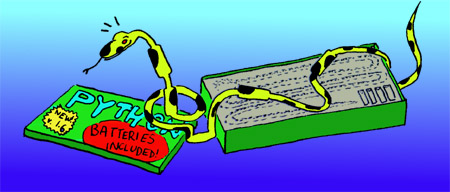
\includegraphics[height=4.5cm]{images/batteries_included.jpg}
\end{frame}

\begin{frame}[fragile]{Mathematics: \texttt{math}}
\begin{itemize}
\item Constants: \texttt{e}, \texttt{pi}
\item Round up/down: \texttt{floor(x)}, \texttt{ceil(x)}
\item Exponential function: \texttt{exp(x)}
\item Logarithm: \texttt{log(x[, base])}, \texttt{log10(x)}
\item Power and square root: \texttt{pow(x, y)}, \texttt{sqrt(x)}
\item Trigonometric functions: \texttt{sin(x)}, \texttt{cos(x)}, \texttt{tan(x)}
\item Conversion degree $\leftrightarrow$ radiant: \texttt{degrees(x)}, \texttt{radians(x)}
\end{itemize}
\begin{lstlisting}[style=Shell]
>>> import math
>>> math.sin(math.pi)
1.2246063538223773e-16
>>> math.cos(math.radians(30))
0.86602540378443871
\end{lstlisting}
\end{frame}


\begin{frame}[fragile]{Random Numbers: \texttt{random}}
\begin{itemize}
\item Random integers: \\ \texttt{randint(a, b)},  \texttt{randrange([start,] stop[, step])}
\item Random floats (uniform distr.): \texttt{random()}, \texttt{uniform(a, b)}
\item Other distibutions: \texttt{expovariate(lambd)}, \texttt{gammavariate(alpha, beta)}, \texttt{gauss(mu, sigma)}, \dots
\item Random element of a sequence: \texttt{choice(seq)}
\item Several unique, random elements of a sequence: \texttt{sample(population, k)}
\item Shuffled sequence: \texttt{shuffle(seq[, random])}
\end{itemize}
\begin{lstlisting}[style=Python]
>>> s = [1, 2, 3, 4, 5]
>>> random.shuffle(s)
>>> s
[2, 5, 4, 3, 1]
>>> random.choice("Hello world!")
'e'
\end{lstlisting}
\end{frame}


\begin{frame}[fragile]{Exact decimals: \texttt{fractions}}

\begin{lstlisting}
>>> from fractions import Fraction
>>> a = Fraction(2, 3)
>>> b = Fraction(2, 5)
>>> print float(a), float(b)
0.66666666666666663 0.40000000000000002
>>> a+b
Fraction(16, 15)
>>> a/b
Fraction(5, 3)
\end{lstlisting}

(See also: module \texttt{decimal}.)
\end{frame}


\begin{frame}[fragile]{Date and Time: \texttt{datetime}}
Date and time objects:
\begin{lstlisting}
d1 = datetime.date(2008, 3, 21)  
d2 = datetime.date(2008, 6, 22)
dt = datetime.datetime(2011, 8, 26, 12, 30)
t = datetime.time(12, 30)
\end{lstlisting}
Calculating with date and time:
\begin{lstlisting}
print d1 < d2
delta = d2 - d1
print delta.days
print d2 + datetime.timedelta(days=44)
\end{lstlisting}
\end{frame}

\begin{frame}[fragile]{More Data Types: \texttt{collections}}
\alert{defaulttict}: Dictionary which creates default values for non-existant keywords:
\begin{lstlisting}
frequency = defaultdict(lambda: 0)

for c in "Hello world!":
    frequency[c] += 1
\end{lstlisting}
Paramter (optional): function creating the default values
\end{frame}


\begin{frame}[fragile]{Operations on Path Names: \texttt{os.path}}
\begin{itemize}
\item Paths: \texttt{abspath(path)}, \texttt{basename(path)}, \texttt{normpath(path)}, \texttt{realpath(path)}
\item Construct paths: \texttt{join(path1[, path2[, ...]])}
\item Split paths: \texttt{split(path)}, \texttt{splitext(path)}
\item File information: \texttt{isfile(path)}, \texttt{isdir(path)}, \texttt{islink(path)}, \texttt{getsize(path)}, \dots
\item Expand home directory: \texttt{expanduser(path)}
\item Expand environment variables: \texttt{expandvars(path)}
\end{itemize} 
\begin{lstlisting}[style=Shell]
>>> os.path.join("spam", "eggs", "ham.txt")
'spam/eggs/ham.txt'
>>> os.path.splitext("spam/eggs.py")
('spam/eggs', '.py')
>>> os.path.expanduser("~/spam")
'/home/rbreu/spam'
>>> os.path.expandvars("/blah/$TEST")
'/bla/test.py'
\end{lstlisting}%$
\end{frame}

\begin{frame}[fragile]{Files and Directories: \texttt{os}}
\begin{itemize}
\item Working directory: \lstinline{getcwd()}, \lstinline{chdir(path)}
\item Changing file permissions: \lstinline{chmod(path, mode)}
\item Changing ower: \lstinline{chown(path, uid, gid)}
\item Creating directories: \lstinline{mkdir(path[, mode])}, \lstinline{makedirs(path[, mode])}
\item Removing files: \lstinline{remove(path)}, \lstinline{removedirs(path)}
\item Renaming files: \lstinline{rename(src, dst)}, \lstinline{renames(old, new)}
\item List of files in a directory: \lstinline{listdir(path)}
\end{itemize}
\begin{lstlisting}[style=Python]
for myfile in os.listdir("mydir"):
    os.chmod(os.path.join("mydir", myfile), 
             stat.S_IRUSR|stat.S_IWUSR)
\end{lstlisting}
\end{frame} 

\begin{frame}[fragile]{Directory Listing: \texttt{glob}}
List of files in a directory with Unix-like extension of wildcards: \texttt{glob(path)}
\begin{lstlisting}[style=Shell]
>>> glob.glob("python/[a-c]*.py")
['python/confitest.py',
 'python/basics.py',
 'python/curses_test2.py',
 'python/curses_keys.py',
 'python/cmp.py',
 'python/button_test.py',
 'python/argument.py',
 'python/curses_test.py']
\end{lstlisting}
\end{frame}

\begin{frame}[fragile]{Files and Directories: \texttt{shutil}}
Higher level operations on files and direcories.
\begin{itemize}
\item Copying files: \texttt{copyfile(src, dst)}, \texttt{copy(src, dst)}
\item Recursive copy: \texttt{copytree(src, dst[, symlinks])}
\item Recursive removal: \\\texttt{rmtree(path[, ignore\_errors[, onerror]])}
\item Recursive move: \texttt{move(src, dst)}
\end{itemize}
\begin{lstlisting}[style=Python]
shutil.copytree("spam/eggs", "../beans", 
                 symlinks=True)
\end{lstlisting}
\end{frame}

\begin{frame}[fragile]{Run Processes: \texttt{subprocess}}
Simple execution of a program:
\begin{lstlisting}[style=Python]
p = subprocess.Popen(["ls", "-l", "mydir"])
returncode = p.wait() # wait for p to end
\end{lstlisting}
Access to the program's output:
\begin{lstlisting}[style=Python]
p = Popen(["ls"], stdout=PIPE, stderr=STDOUT) 
p.wait()
output = p.stdout.read()
\end{lstlisting}
Pipes between processes (\lstinline{ls -l | grep txt})
\begin{lstlisting}[style=Python]
p1 = Popen(["ls", "-l"], stdout=PIPE)
p2 = Popen(["grep", "txt"], stdin=p1.stdout)
\end{lstlisting}
\end{frame}

\begin{frame}[fragile]{Access to Command Line Parameters: \texttt{optparse}}
\begin{itemize}
\item Simple list of parameters: $\rightarrow$ \texttt{sys.argv}
\item More convenient for handling several options: \texttt{OptionParser}
\end{itemize}
\begin{lstlisting}[style=Python]
parser = optparse.OptionParser()
parser.add_option("-f", "--file", 
                  dest="filename",
                  default="out.txt",
                  help="output file")
parser.add_option("-v", "--verbose",
                  action="store_true", 
                  dest="verbose", 
                  default=False,
                  help="verbose output")

(options, args) = parser.parse_args()
print options.filename, options.verbose
print args
\end{lstlisting}
\end{frame}
\begin{frame}[fragile]{Zugriff auf Kommandozeilenparameter: \texttt{optparse}}
Usage of an optparse program:
\begin{lstlisting}[style=Shell]
$ ./test.py -h
usage: test.py [options]

options:
  -h, --help     show this help message and exit
  -f FILENAME, --file=FILENAME
                 output file
  -v, --verbose  verbose output
\end{lstlisting} %$
\begin{lstlisting}[style=Shell]
$ ./test.py -f aa bb cc
aa False
['bb', 'cc']
\end{lstlisting} %$
\end{frame}

\begin{frame}[fragile]{Configuration Files: \texttt{ConfigParser}}
Simple format to store configuration etc: Windows' INI format
\begin{lstlisting}[style=Python]
[font]
font = Times New Roman
# comment (or: ! as comment symbol)
size = 16

[colors]
font = black
pointer = %(font)s
background = white
\end{lstlisting}
\end{frame}

\begin{frame}[fragile]{Configuration Files: \texttt{ConfigParser}}
Reading configuration files:
\begin{lstlisting}[style=Python]
parser = ConfigParser.SafeConfigParser()
parser.readfp(open("config.ini", "r"))
print parser.get("colors", "font")
\end{lstlisting}
More parser methods:
\begin{itemize}
\item List of all sections: \texttt{sections()}
\item List of all options: \texttt{options(section)}
\item List of all options and values: \texttt{items(section)}
\item Reading values: \texttt{get(sect, opt)}, \\
\texttt{getint(sect, opt)}, \texttt{getfloat(sect, opt)}, \texttt{getboolean(sect, opt)}
\end{itemize}
\end{frame}

\begin{frame}[fragile]{Config Files: \texttt{ConfigParser}}
Writing configuration files:
\begin{lstlisting}[style=Python]
parser = ConfigParser.SafeConfigParser()
parser.add_section("colors")
parser.set("colors", "font", "black")
parser.write(open("config.ini", "w"))
\end{lstlisting}
More parser methods:
\begin{itemize}
\item Adding a section: \texttt{add\_section(section)}
\item Deleting a section: \texttt{remove\_section(section)}
\item Adding an option: \texttt{set(section, option, value)}
\item Removing and option: \texttt{remove\_option(section, option)}
\end{itemize}
\end{frame}

\begin{frame}[fragile]{CSV Files: \texttt{csv}}
CSV: Comma Seperated Values
\begin{itemize}
\item Data tables in ASCII format
\item Columns are delimited by a predefined character (most often comma)
\end{itemize}
\begin{lstlisting}[style=Python]
reader = csv.reader(open("test.csv", "rb"))
for row in reader:
    for item in row: 
        print item
\end{lstlisting}
\begin{lstlisting}[style=Python]
writer = csv.writer(open(outfile, "wb"))
writer.writerow([1, 2, 3, 4])
\end{lstlisting}
\end{frame}

\begin{frame}[fragile]{CSV Files: \texttt{csv}}
Handling different kinds of formats (dialects):
\begin{lstlisting}[style=Python]
reader(csvfile, dialect='excel') # Default
writer(csvfile, dialect='excel_tab')
\end{lstlisting}
\vspace*{3mm}
Specifying individual format parameters:
\begin{lstlisting}[style=Python]
reader(csvfile, delimiter=";")
\end{lstlisting}
Further format parameters: \texttt{lineterminator}, \texttt{quotechar}, \texttt{skipinitialspace}, \dots
\end{frame}

\begin{frame}[fragile]{Serialising Objects: \texttt{pickle}}
Saving single, arbitrary objects in files:
\begin{lstlisting}[style=Python]
obj = {"hello": "world", "spam":1}
pickle.dump(obj, open("blah.bin", "wb"))
# ...
obj = pickle.load(open("blah.bin", "rb"))
\end{lstlisting}
Converting objects in strings (e.g. to send via streams):
\begin{lstlisting}[style=Python]
s = pickle.dumps(obj)
# ...
obj = pickle.loads(s)
\end{lstlisting}
\end{frame}

\begin{frame}[fragile]{Persistent Dictionaries: \texttt{shelve}}
A shelve is used like a dictionary; it saves its content to a file.
\begin{lstlisting}[style=Python]
d = shelve.open("blah")
d["spam"] = "eggs"
d["blah"] = 1
del d["foo"]   
d.close()  
\end{lstlisting}
\end{frame}

\begin{frame}[fragile]{Lightweight Database: \texttt{sqlite3}}
Database in a file or in memory; in Python's stdlib sine 2.5.
\begin{lstlisting}[style=Python]
conn = sqlite3.connect("bla.db")
c = conn.cursor()

c.execute("""CREATE TABLE Friends
             (firstname TEXT, lastname TEXT)""")
c.execute("""INSERT INTO Friends
             VALUES("Jane", "Doe")""")
conn.commit()
\end{lstlisting}
\begin{lstlisting}[style=Python]
c.execute("""SELECT * FROM Friends""")
for row in c: print row

c.close(); conn.close()
\end{lstlisting}
\end{frame}

\begin{frame}[fragile]{Lightweight Database: \texttt{sqlite3}}
String formatting is insecure since it allows injection of arbitrary SQL code!
\begin{lstlisting}[style=Python]
# Never do this!
symbol = "Jane"
c.execute("... WHERE firstname = '%s'" % symbol)
\end{lstlisting}
\vspace{2mm}

\includegraphics[width=\textwidth]{images/exploits_of_a_mom.png}
\end{frame}

\begin{frame}[fragile]{Lightweight Database: \texttt{sqlite3}}
Instead: Use the placeholder the database API provides:
\begin{lstlisting}[style=Python]
c.execute("... WHERE name = ?", symbol)
\end{lstlisting}
\begin{lstlisting}[style=Python]
f = (("Janis", "Joplin"), ("Bob", "Dylan"))
for item in friends:
    c.execute("""INSERT INTO Friends 
                 VALUES (?,?)""", item)
\end{lstlisting}
\end{frame}

\begin{frame}[fragile]{Tar Archives: \texttt{tarfile}}
Extracting a tgz:
\begin{lstlisting}[style=Python]
tar = tarfile.open("spam.tgz")
tar.extractall()
tar.close()
\end{lstlisting}
\vspace*{3mm}
Creating a tgz:
\begin{lstlisting}[style=Python]
tar = tarfile.open("spam.tgz", "w:gz")
tar.add("/home/rbreu/test")
tar.close()
\end{lstlisting}
\end{frame}

\begin{frame}[fragile]{Logging Output: \texttt{logging}}
Flexible output of information which can be easily customised.
\begin{lstlisting}[style=Python]
import logging
logging.debug("Very special information.")
logging.info("I am doing this and that.")
logging.warning("You should know this.")
\end{lstlisting}
\begin{lstlisting}[style=shell]
WARNING:root:You should know this.
\end{lstlisting}
\begin{itemize}
\item Messages are assigned a priority:\\
 \texttt{CRITICAL}, \texttt{ERROR}, \texttt{WARNING}, \texttt{INFO}, \texttt{DEBUG}
\item Default: Only messages with priority \texttt{WARNING} or higher are printed
\end{itemize}
\end{frame}

\begin{frame}[fragile]{Logging Output: \texttt{logging}}
Example: Output into file, custom format, higher logging level:
\begin{lstlisting}[style=Python, basicstyle=\ttfamily\small]
logging.basicConfig(level=logging.DEBUG,
  format="%(asctime)s %(levelname)-8s %(message)s",
  datefmt="%Y-%m-%d %H:%M:%S",
  filename='/tmp/spam.log', filemode='w')
\end{lstlisting}
\begin{lstlisting}[style=Shell, basicstyle=\ttfamily\small]
$ cat /tmp/spam.log
2007-05-07 16:25:14 DEBUG   Very special information.
2007-05-07 16:25:14 INFO    I am doing this and that.
2007-05-07 16:25:14 WARNING You should know this.
\end{lstlisting} %$
You can use multiple logger instancdes at the same time, see Python documentation.
\end{frame}

\begin{frame}[fragile]{Regul"are Ausdr"ucke: \texttt{re}}
Einfaches Suchen nach Mustern:
\begin{lstlisting}[style=Shell]
>>> re.findall(r"\[.*?\]", "a[bc]g[hal]def")
['[bc]', '[hal]']
\end{lstlisting}
\vspace*{2mm}
Ersetzen von Mustern:
\begin{lstlisting}[style=Shell]
>>> re.sub(r"\[.*?\]", "!", "a[bc]g[hal]def")
'a!g!def'
\end{lstlisting}
\vspace*{2mm}
Wird ein Regex-Muster mehrfach verwendet, sollte es aus Geschwindigkeitsgr"unden compiliert werden:
\begin{lstlisting}[style=Shell]
>>> pattern = re.compile(r"\[.*?\]")
>>> pattern.findall("a[bc]g[hal]def")
['[bc]', '[hal]']
\end{lstlisting}
\end{frame}

\begin{frame}[fragile]{Regul"are Ausdr"ucke: \texttt{re}}
Umgang mit Gruppen:
\begin{lstlisting}[style=Shell]
>>> re.findall("(\[.*?\])|(<.*?>)", 
               "[hi]s<b>sdd<hal>")
[('[hi]', ''), ('', '<b>'), ('', '<hal>')]
\end{lstlisting}
\vspace*{2mm}
Flags, die das Verhalten des Matching beeinflussen:
\begin{lstlisting}[style=Shell]
>>> re.findall("^a", "abc\nAbc", re.I|re.M)
>>> ['a', 'A']
\end{lstlisting}
\begin{itemize}
\item \texttt{re.I}: Gro"s-/Kleinschreibung ingnorieren
\item \texttt{re.M}: \lstinline{^} bzw. \lstinline{$} matchen am Anfang/Ende jeder Zeile (nicht nur am Anfang des Strings) %$
\item \texttt{re.S}: \lstinline{.} matcht auch Zeilenumbruch
\end{itemize}
\end{frame}


\begin{frame}[fragile]{URLs lesen: \texttt{urllib2}}
Einfaches lesen:
\begin{lstlisting}
import urllib2
r = urllib2.urlopen('http://www.fz-juelich.de')
print r.read()
print r.headers["content-type"]
\end{lstlisting}
Man kann den Request vorm Absenden anpassen:
\begin{lstlisting}
opener = urllib2.build_opener()
opener.addheaders = [('User-agent', 
                      'Mozilla/5.0')]
r = opener.open('http://www.fz-juelich.de')
\end{lstlisting}
Es werden Cookies, Authentifizierung, Proxies etc unterst"utzt.
\end{frame}


\begin{frame}[fragile]{XML-RPC-Client: \texttt{xmlrpclib}}
\begin{itemize}
\item XML-RPC: \alert{Remote Procedure Call} via XML und HTTP
\item unabh"anging von Plattform und Programmiersprache
\end{itemize}
\begin{lstlisting}[style=Python]
import xmlrpclib

s = xmlrpclib.Server("http://localhost:8000")
print s.add(2,3) 
print s.sub(5,2) 
\end{lstlisting}
Konvertierungen f"ur die g"angigen Datentypen geschehen automatisch: 
Booleans, Integer, Floats, Strings, Tupel, Listen, Dictionaries mit Strings als Keys, \dots
\end{frame}

\begin{frame}[fragile]{XML-RPC-Server: \texttt{SimpleXMLRPCServer}}
\begin{lstlisting}[style=Python]
from SimpleXMLRPCServer import SimpleXMLRPCServer

# Methoden, die der Server zur Verfuegung
# stellen soll:
class MyFuncs:
    def add(self, x, y):
        return x + y
    def sub(self, x, y):
        return x - y
    
# Erstelle und starte Server:
server = SimpleXMLRPCServer(("localhost", 8000))
server.register_instance(MyFuncs())
server.serve_forever()
\end{lstlisting}
\end{frame}


